\chapter{Methodology}

\section{First-Principles Calculations}

In this dissertation, the ground state energy structures, thermodynamic properties and mechanical properties were calculated using first-principles based on Density Functional Theory. The first-principles refers to the calculations originating from "first-principles", meaning that the inputs were the atomic coordinates and atomic numbers. This method computes the interactions between atoms in a periodic supercell. This was determined using quantum mechanical electronic theory that is based on the electronic charge density and does not rely on any empirical data. This section provides a description of the DFT methodology.

Schr$\ddot{o}$dinger's time-independent non-relativistic equation is a solution to the many-body problem of calculating the interactions of positively charged nuclei and negatively charged electrons. The Schr$\ddot{o}$dinger equation is:

%%
\begin{equation}
\label{eq: schrodinger}
\left[ \sum_{i=1}^{N} \left( - \frac{\hbar^2}{2m} \nabla_{i}^2 + V_{ext} (r_{i}) \right) + \sum_{i<j} U (r_{i}, r_{j}) \right] \Psi = E_{s} \Psi
\end{equation}
%%

\noindent where the first bracketed part represents the Hamiltonian ($\hat{H}$), $\Psi$ describes the wave function of electrons, $E_{s}$ describes the systems energy. The $\hat{H}$ of the system is described by three parts, the first part represents the kinetic energy with $N$ being the total number of electrons in the system, $\hbar$ being Planck's constant and $m$ the mass of an electron. The second term $V_{ext}$ gives the external potential and $U$ is the potential of the electron-electron repulsion.

Eq. \ref{eq: schrodinger} can be solved for $\Psi$ with the lowest energy $E_s$ being the ground state energy, assuming the nuclei-nuclei interactions are neglected due to the Born-Oppenheimer approximation. The Born-Oppenheimer approximation allows us to assume the nuclei are stationary and ignore the motion of the nuclei on the electronic timescale, due to the mass difference, with nuclei being $\sim$ 10$^3$ to 10$^5$ larger than electrons. However, even with this approximation solving Eq. \ref{eq: schrodinger} is difficult to deal with due to the electron-electron Columb interactions making the electronic motion correlated and the fact that the many-body problem results in too many variables because there are 3N degrees of freedom. 

Hohenberg-Kohn formulated two theorems to simplify this problem \cite{Hohenberg1964}. The first theorem states that the external potential is a unique functional of the electron density. The second theorem states that the density that minimizes the total energy is the exact ground state density and thus the ground state is obtained variationaly. With these theorems, Kohn-Sham proved that the problem can be solved as if the electrons are not interacting and still obtain the density as if they were, by \cite{Kohn1965}:
 
  \begin{equation}
 \label{eq: kohnsham}
\left[ -\frac{\hbar^2}{2m} \nabla^{2} + V_{ext} (r) + V_{Hartree}(r) + V_{XC} (r) \right] \phi_{1}(r) = \epsilon_{i} \psi_{i}(r)
 \end{equation}
 %%
 
 \noindent where $V_{ext}(r)$ describes the electron-nuclei interaction similar as in Eq. \ref{eq: schrodinger}:

\begin{equation}
\label{eq: vext}
V_{ext} = - e^2 \sum_{a} \frac {Z_{a}}{|r_i - R_a|}
\end{equation}

\noindent where $r_i$ represents the position of electron $i$ and $R_a$ represents the position of nucleus $a$ with a charge valance of $Z_a$. The electron-electron interactions are represented by $V_{Hartree}$:

\begin{equation}
\label{eq: vhartree}
V_{Hartree} (r) = e^{2} \int \frac {\rho(r)}{|r - r_{j}|} d^3r
\end{equation}
%%

\noindent where $r$ and $r_j$ represent the electrons and $\rho (r)$ is described by :

\begin{equation}
\label{eq: rhop}
\rho (r) = \sum_{i}^N | \psi_{i} (r) |^2
\end{equation}
%%

\noindent The final term of $V_{xc}$ is the exchange correlation potential that is described in terms of an exchange-correlation energy. While there is no exact solution to the exchange-correlation (X-C) energy available, there are multiple different approximations. Each approximation is done to account for different things. In the present work, the generalized gradient approximation by Perdew and Wang (PW91) \cite{Perdew1992} and the generalized gradient approximation by Perdew, Burke and Ernzerhoff (PBE) \cite{Perdew1996a} where used. The generalized gradient approach improves the total energies, atomization energies as opposed to other methods such as the local density approximation \cite{Ceperley1980} but can over-correct for the expansion and softening of bonds. The generalized gradient approximation (GGA) is favored for densities that are inhomogeneous. Based on previous research done by Perdew et al. \cite{Perdew1996a}, GGA's are considered to be adequate approximations for calculating metals \cite{Perdew1996a}. The use of PW91 vs PBE was compared when looking at the elastic properties of the Ti-Ta system in Figure \ref{Ch2-figure:PBEvsPW91}. The results showed little difference in calculated elastic properties. The PW91 X-C functional was designed to satisfy as many exact conditions as possible and thus has some issues. Perdew introduced the PBE X-C functional as an improvement to PW91 which satisfied less exact conditions and only looked at the ones that were energetically significant for metals. Due to this and the fact the results vary so little, the PBE X-C functional was chosen to be used for the present thesis work. By implementing the theorems and the Kohn-Sham equation, the energy of the system can thus be calculated.

\subsection{Density Functional Theory at 0 $^\circ$K}

 The ground state energy at 0 $^\circ$K without the contribution of zero-point vibrational energy was calculated by using the equation of states (EOS) fitting for the relationship between the energy and volume of the structure. The EOS fitting was achieved through an energy-volume ($E_{0}-V$) curve of 5 or more relaxed volumes and using the four-parameter Birch-Murnaghan (BM4) EOS \cite{Shang2010}:

%%
\begin{equation}
\label{eq: zeroenergy}
E_{0}(V) = a + bV^{\frac{-2}{3}} + cV^{{-4}{3}} + dV^{-2}
\end{equation}
%%

\noindent where $a$, $b$, $c$ and $d$ are fitting parameters. From this, the volume $V_0$, ground state energy $E_{0}$, bulk modulus $B_{EOS}$, and first derivative with respect to pressure $B'_{EOS}$ can be calculated. 

From the ground state energies, the energy of formation and enthalpy of formation at 0 $^\circ$K was calculated by finding the difference between the structures energy and a reference state, normally the standard element reference (SER) state at standard pressure and temperature. The valance configuration for each element was selected based on the VASP recommendations. The p electrons were treated as valance for the Mo and Ta, the d electrons were treated as valance for Sn and the s electrons were treated as valance for Ti, Nb, and Zr \cite{Kresse1996,Kresse1999}.

\subsection{Finite-temperature thermodynamics}

The Helmholtz energy, $F(V,T)$ was calulated, with DFT, as a function of temperature $T$ and volume $V$:
 %%
 \begin{equation}
 \label{eq: helmholtz}
 F(V,T) = E_{0}(V) + F_{vib}(V,T) + F_{T-el}(V,T)
 \end{equation}
 %%
 
\noindent where $E_0$ is the static contribution at 0 $^\circ$K calculated from Eq. \ref{eq: zeroenergy}, $F_{vib}$ is the temperature-dependent vibrational contribution, and $F_{T-el}$ is the thermal electronic contribution. At ambient pressure, the Helmholtz energy of the system is equal to the Gibbs energy, which is used in the CALPHAD modeling. The vibrational contribution was obtained through the phonon quasiharmonic supercell (phonon approach) or the Debye-Gr\"uneisen method (Debye). The phonon approach is a more accurate approach compared to the Debye model but it is also more computationally expensive. In the present work, both the phonon and Debye models are used in different sections. The vibrational contribution obtained through phonon calculations of at least five different volumes is expressed by \cite{Wang2012}:

%%
\begin{equation}
\label{eq: phonon}
F_{vib}(V,T) = k_{b}T \int_{0}^{\infty} ln \left[ 2sinh \frac{\hbar \varrho}{2k_BT} \right] g(\varrho) d\varrho
\end{equation}
%%

\noindent where $g(\varrho)$ is the phonon density of states as a function of phonon frequency $\varrho$ at volume $V$. $\varrho$ is normally expressed in literature as $\omega$, however, due to the extensive discussion of the $\omega$ phase in this work the phonon frequency is expressed as $\varrho$ to avoid confusion. In addition, the Debye model is used to estimate the vibrational contribution \cite{Shang2010}: 

%%
\begin{equation}
\label{eq: debye}
F_{vib}(V,T) = \frac{9}{8} k_{b} \theta_{D}(V) + k_{B}T \left[ 3 ln \left( 1 - e^{\frac{-\theta_{D}}{T}} \right) - D \left( \frac{\theta_D}{T} \right) \right] 
\end{equation}
%%

\noindent where $\theta_{D}$ is the Debye temperature, $T$ is the temperature, and $D \left[ \frac{\theta_{D}}{T} \right] $ is the Debye function. $\theta_{D}$ is calculated through: 

%%
\begin{equation}
\label{eq: debyetemp}
\theta_{D} = s \frac{(6\pi^2)^{\frac{1}{3}}\hbar}{k_B} V_{0}^{\frac{1}{6}} \left( \frac{B}{M} \right)^{\frac{1}{2}} \left( \frac{V_0}{V} \right)^{\gamma} 
\end{equation}
%%

\noindent where $s$ is the Debye temperature scaling factor, $\gamma$ is the Gr$\ddot{u}$neisen parameter determined by the pressure derivative of bulk modulus ($B'_{EOS}$), $B_{EOS}$ is the bulk modulus, $M$ is the atomic mass, and $V_0$ is the equilibrium volume. Here the equilibrium properties $V_0$, $B_{EOS}$, and $B'_{EOS}$ are estimated from the EOS of Eq. \ref{eq: zeroenergy}. The Debye temperature scaling factor was determined by Moruzzi et al. \cite{Moruzzi1988} to be 0.617 for nonmagnetic metals. However, this value has been shown to be less accurate for other materials. Liu et al. extensively looked at the Debye scaling factor and how to calculate the scaling factor based on the Poisson's ratio of a material \cite{Liu2015}. The methodology by Liu et al. \cite{Liu2015} was used for the present work to calculate the scaling factor: 

%%
\begin{equation}
\label{eq: debyescaling}
s(\nu) = 3^{\frac{5}{6}} \left[ 4\sqrt{2} \left( \frac{1 + \nu}{1 - \nu} \right)^{\frac{3}{2}} + \left( \frac{1 + \nu}{1 - \nu} \right)^{\frac{-1}{3}} \right]
\end{equation}
%%

\noindent where $\nu$ is the Poisson's ratio, which can be calculated from the elastic stiffness constants.

The thermal electronic contribution is based on the electronic density of states and calculated with the Fermi-Dirac statistics \cite{Shang2010,Wang2004}:

%%
\begin{equation}
\label{eq:thermalelectronic}
F_{T-el} = E_{T-el} - T S_{T-el}
\end{equation}
%%

\noindent The $E_{T-el}$ and $S_{T-el}$ represent the energy and entropy of the thermal electron excitations, respectively. The $E_{T-el}$ is expressed by:

%%
\begin{equation}
\label{eq:etel}
E_{T-el} (V,T) = \int n\left(\epsilon, V\right) f \left(\epsilon, T\right) \epsilon d \epsilon - \int^{\epsilon_{f}} n (\epsilon) \epsilon d \epsilon
\end{equation}
%%

\noindent and the entropy $S_{T-el}$ is expressed by:

%%
\begin{equation}
\label{eq:sel}
S_{T-el} (V,T) = -k_{B} \int n(\epsilon, V) \left[ ln f \left(\epsilon,T\right) + \left( 1 - f(\epsilon, T) \right) ln \left( 1 - f \left(\epsilon, T \right) \right) \right] d\epsilon 
\end{equation}
%%

\noindent where $n(\epsilon, V)$ is the electronic density of states (DOS) at energy $\epsilon$,  $f (\epsilon,T)$ is the Fermi-Dirac distribution, $\epsilon_{f}$ is the Fermi energy level and $k_{B}$ is Boltzmann's constant. The Fermi-Dirac distribution $f (\epsilon, T)$ is expressed by:

%%
\begin{equation}
\label{eq:fermidirac}
f (\epsilon,T) = \left[ exp \left( \frac{\epsilon - \mu}{k_{B} T} \right) + 1 \right]^{-1}
\end{equation}
%%

\noindent and $\mu$ is the chemical potential of the electrons. 


\subsection{Elastic stiffness calculations}

The single crystal elastic stiffness constants ($c_{ij}$$'s$) were calculated from the ground state energy structure using a stress-strain method developed by Shang et al. \cite{Shang2007c}. With this method, a set of independent strains $\varepsilon = (\varepsilon_{1}, \varepsilon_{2}, \varepsilon_{3}, \varepsilon_{4}, \varepsilon_{5}, \varepsilon_{6})$ were imposed on the crystal lattice, where $\varepsilon_{1}$, $\varepsilon_{2}$, and $\varepsilon_{3}$ are the normal strains, $\varepsilon_{4}$, $\varepsilon_{5}$, and $\varepsilon_{6}$ the shear strains, and a set of stresses $\sigma = (\sigma_{1}, \sigma_{2}, \sigma_{3}, \sigma_{4}, \sigma_{5},\sigma_{6})$ were generated. Hooke's law is then used to calculate the elastic stiffness constants: 

%%
\begin{equation}
\label{eq: hookes}
\begin{pmatrix}
	c_{11} & c_{12} & c_{13} & 0 & 0 & 0\\
	c_{12} & c_{22} & c_{23} & 0 & 0 & 0\\
	c_{13} & c_{23} & c_{33} & 0 & 0 & 0\\
	0 & 0 & 0 & c_{44} & 0 & 0\\
	0 & 0 & 0 & 0 &  c_{55} & 0\\
	0 & 0 & 0 & 0 & 0 & c_{66} \\    		
\end{pmatrix} =
\begin{pmatrix}
	\varepsilon_{1,1} & & \varepsilon_{1,n}\\
	\varepsilon_{2,1} & & \varepsilon_{2,n}\\
	\varepsilon_{3,1} & ... & \varepsilon_{3,n}\\
	\varepsilon_{4,1} & & \varepsilon_{4,n}\\
	\varepsilon_{5,1} & & \varepsilon_{5,n}\\
	\varepsilon_{6,1} & & \varepsilon_{6,n}\\					
\end{pmatrix}^{-1}
\begin{pmatrix}
	\sigma_{1,1} & & \sigma_{1,n}\\
	\sigma_{2,1} & & \sigma_{2,n}\\
	\sigma_{3,1} & ... & \sigma_{3,n}\\
	\sigma_{4,1} & & \sigma_{4,n}\\
	\sigma_{5,1} & & \sigma_{5,n}\\
	\sigma_{6,1} & & \sigma_{6,n}\\					
\end{pmatrix}
\end{equation}
%%

\noindent where "-1" represents the pseudo-inverse. Due to symmetry, the bcc structure only has three independent elastic stiffness constants. However, with a lack of bcc stability for some of the calculations, all of the elastic stiffness constants were calculated and the average $\overline{C}_{11}$, $\overline{C}_{12}$ and $\overline{C}_{44}$ values were used:

%%
\begin{equation}
\label{eq: averagec11}
\overline{C}_{11} = \frac{(c_{11} + c_{12} + c_{44})}{3}
\end{equation}
%%

%%
\begin{equation}
\label{eq: averagec12}
\overline{C}_{12} = \frac{(c_{12} + c_{13} + c_{23})}{3}
\end{equation}
%%

%%
\begin{equation}
\label{eq: averagec44}
\overline{C}_{44} = \frac{(c_{44} + c_{55} + c_{66})}{3}
\end{equation}
%%

\noindent This case is for the unstable bcc elastic calculations to mimic the behavior of a cubic structure. The largest variance between the similar elastic stiffness constants, when calculating the average, was used to show the deviation from the bcc symmetry in the calculations, shown as error bars. The stable bcc structures show no variance and thus no error bars. To examine the effects of different strain on the elastic properties, three groups of non-zero strain magnitudes, $\pm$0.01, $\pm$0.03, and $\pm$0.07, were tested in chapter 5 and it can be noted that the results have negligible changes with respect to the three groups of strains tested herein. Therefore, $\pm$0.01 was used for all the calculations. The polycrystalline elastic properties including bulk ($B$), shear ($G$), and $E$ modulus were calculated from the elastic stiffness constants, based on the Voigt-Reuss-Hill approach \cite{Simmons1971b}. The Voigt gives the upper elastic bound due to the assumption of constant strain in all grains, the Reuss gives the lower elastic bound due to the assumption of constant stress in all grains, and the Hill approach is the average of Voigt and Reuss and is closer to real case \cite{Zuo1993,Chung1967}. The Hill approach is hence what is listed in the results section. The Voigt and Reuss bounds were also plotted in the figures to give the bounds of the moduli values.

In order to fully investigate the effects of the alloying elements on the Ti-alloys, the mechanical stability of the bcc phase was studied. The mechanical stability was given by on Born's criteria for a cubic crystal  \cite{Born1998,Nye1985}:


\begin{equation}
\label{eq: born1}
\overline{C}_{11} -|\overline{C}_{12}| > 0
\end{equation}
\begin{equation}
\label{eq: born2}
\overline{C}_{11} + 2\overline{C}_{12} > 0
\end{equation}
\begin{equation}
\label{eq: born3}
\overline{C}_{44} > 0
\end{equation}

\noindent Based on Born's criteria, when$\overline{C}_{11} - \overline{C}_{12}$ becomes negative then the phase, bcc in this case, loses mechanical stability and thus $\overline{C}_{11} - \overline{C}_{12}$ is plotted in the results section.

\subsection{Special quasirandom structures (SQS)}

To calculate the energies, enthalpies of formation and elastic properties across the entire binary and ternary composition range, varying compositions of special quasirandom structures (SQS) were used. The SQS are small supercells used to mimic randomly substituted structures in terms of correlation functions. The binary and ternary bcc SQS, used in the present work, were previously generated by Jiang et al.\cite{Jiang2004,Jiang2009}. The relaxation of these structures is complicated because local atomic relaxations can cause the structure to lose the bcc lattice symmetry. To preserve structural symmetry, the calculations were carried out with different relaxation schemes only alloying the cell shape and cell volume to be relaxed to determine the lowest energy structure. In order to ensure the bcc symmetry was preserved the energies were plotted as a function of composition. Then the symmetry was verified. There are two ways to verify whether the SQS is still bcc or not after the relaxation. The first is to merge different elements into one element for the SQS structure, and then, use codes available to check the symmetry or space group (such as VASP and phonopy codes). The second is to visualize the structure directly using a visualization software such as VESTA and compare the symmetry to the unrelaxed bcc structure. For the present work, the relaxed structures were plotted in the visualization software and compared to the unrelaxed structure. In some cases, even without comparing, it was very obvious that the structure had lost bcc symmetry. For the cases where it wasn't obvious the comparison was done using symmetry codes (VASP, phonopy, etc). After the relaxation, at least five different volume structures are generated and the ions were allowed to relax. This yields the different volumes needed for the EOS fitting described above, which allows a better prediction of the different properties as a function of composition. 

\subsection{High-throughput partition function}

INTRODUCE THE PARITITION FUNCTION APPROACH. The combined potential energy can be calculated by REF:

%%
\begin{equation}
\label{eq: combined_energy}
E_{c} = E_{g} + \sum p_{i} \left( E_{i} - E_{g} \right) 
\end{equation}
%%

\noindent where $E_{g}$ is the ground state energy and $E_{i}$ is the energy of metastable phase $i$. All of the energies were calculated from first-principles based on DFT using the EOS fitting in Eq. \ref{eq: zeroenergy}. $p_{i}$ is expressed by:

%%
\begin{equation}
\label{eq: pi}
p_{i} = \frac{Z_{i}}{Z_{c}} 
\end{equation}
%%

\noindent where $Z_{i}$ and $Z_{c}$ are calculated by:

%%
\begin{equation}
\label{eq: zc}
Z_{c} = \sum_{j} e^{- \frac{E_{c}}{k_{B}T}} 
\end{equation}
%%

\noindent From Eq. \ref{eq: combined_energy}-\ref{eq: zc} the combined Helmholtz energy is calculated by:

%%
\begin{equation}
\label{eq: combinedhelmholtz}
F_{c} = - k_{B} T \left( \sum \frac{Z_{i}}{Z_{c}} lnZ_{i} - \sum \frac{Z_{i}}{Z_{c}} ln \frac{Z_{i}}{Z_{c}}  \right)
\end{equation}
%%

\noindent From the combined helmholtz the phase fractions MORE

\subsection{First-principles calculation error}

The error between the previous results (experimental or calculation) and present results was calculated using:

%%
\begin{equation}
\label{eq: error}
\sqrt{\frac{\Sigma[(A_{calc}-A{ref})]^{2}}{\kappa}} = Difference
\end{equation}
%%

\noindent where $A_{calc}$ is from the present calculation and $A_{ref}$ is from the previous experiment or calculation, and $\kappa$ is the total number of data points. 

\section{CALPHAD method}

The CALPHAD method evaluates parameters to represent the Gibbs energy of individual phases as a function of temperature, pressure and composition. Thermochemical and phase boundary data obtained from experiments and first-principles calculations were used in the PARROT module of Thermo-Calc to evaluate the thermodynamic interaction parameters \cite{Andersson2002}. The Gibbs free energy is described by enthalpy $H$, temperature $T$ and entropy $S$ as follows:

%%
\begin{equation}
\label{eq: gibbs}
G = H - T S 
\end{equation}
%%

\noindent The Gibbs energy is then parameterized and expressed by:

%%
\begin{equation}
\label{eq: parameterizaiton}
G - H^{SER} = a + bT + cT ln T + d T^2 + \sum_{2}^{n} e_{n} T^{n}
\end{equation}
%%

\noindent where $H^{SER}$ refers to the elemental enthalpy in the SER state and $a$, $b$, $c$, $d$, $e$ are coefficients. Other thermodynamic properties such as, enthalpy, entropy and heat capacity can be derived from this equation. The parameterized equations for the pure elements have been determined and widely adopted from the SGTE to ensure global compatibility between different databases \cite{Dinsdale1991}.

\subsection{Solution phases}

The databases were built upon the pure elements and then the effects of the binary and ternary interactions are modeled. Normally, the effects of alloying are modeled as solution phases or stoichiometric phases. The solution phases with one sublattice were described by: 

%%
\begin{equation}
\label{eq: gibbssolution}
G_m^{\phi} = \sum x_{A} ^{0}G_{A}^{\phi} + R T \sum x_{A} ln x_{A} + ^{XS}G_{m}^{\phi}
\end{equation}
%%

\noindent where $x_{A}$ is the mole fraction of element $A$ and $^{0}G_{A}^{\phi}$ is the molar Gibbs energy of pure element $A$ in the specific phase ($\phi$) being modeled, the second term describes the ideal interaction between elements. The last term represents the excess mixing energy, representing the non-ideal interactions between species $A$ and $B$. The excess mixing energy can be expressed by the Redlich-Kister polynomial as \cite{Redlich1948b}: 

%%
\begin{equation}
\label{eq: gibbexsol}
^{XS}G_m^{\phi} = \sum x_{A} x_{B} \sum_{k=0} ^{k}L_{A,B}^{\phi} (x_{A} - x_{B})^k
\end{equation}
%%

\noindent where $^kL_{A,B}^{\phi}$ represents the interaction parameter for elements $A$ and $B$ in phase $\phi$ described by:

%%
\begin{equation}
\label{eq: binip}
L_{A,B}^{\phi} = ^{k}a + ^{k}bT
\end{equation}
%%

\noindent in which $^{k}a$ and $^{k}b$ are evaluated model parameters. Eq. \ref{eq: gibbexsol} can be extended to multi-component systems as:

%%
\begin{multline}
\label{eq: gibbexsolmulti}
^{XS}G_m^{\phi} = \sum x_{A} x_{B} \sum_{k=0} ^{k}L_{A,B}^{\phi} (x_{A} - x_{B})^k + \sum x_{A} x_{B} x_{C} \\ \left[ ^{0}L_{A, B, C}^{\phi} (x_{A} + \delta_{A, B, C} + ^{1}L_{A, B, C}^{\phi} (x_{B} + \delta_{A, B, C} + ^{2}L_{A, B, C}^{\phi} (x_{c} + \delta_{A, B, C} ) \right]
\end{multline}
%%

\noindent where the ternary interaction parameters $L_{A, B, C}^{\phi}$ are described the same as the binary interaction parameters in Eq. \ref{eq: binip} and $\delta_{A, B, C}$ is defined as $\delta_{A, B, C} = ( 1 - x_{A} - x_{B} - x_{C})/3$

In the present thesis, while no order-disorder modeling was done, the order-disorder model was used in many of the previous models evaluated. At low temperatures in many of the Ti-containing binary alloys, the randomly substituted bcc-A2 phase goes through a second order transition to become the ordered simple cubic B2 phase (CsCl-type). This modeling was discussed extensively in the COST 507 by Ansara \cite{Ansara1998}. 

\subsection{Stoichiometric compounds}

The Gibbs energy of stoichiometric compounds was modeled in per mole unit formula. For the stoichiometric compound, $A_{p}B_{q}$, the Gibbs energy is expressed by \cite{Zacherl2012}: 

%%
\begin{equation}
\label{eq: stoichiometric}
^{0}G_{m}^{A_{p}B_{q}} = a + bT + p * ^{0}G_{A}^{SER} + q * ^{0}G_{B}^{SER}
\end{equation}
%%

\noindent where $a$ and $b$ are the evaluated parameters, $^{0}G_{A}^{SER}$ is the Gibbs energy of pure element $A$ in the SER phase, $^{0}G_{B}^{SER}$ is the Gibbs energy of pure element $B$ in the SER phase, $p$ is the number of atoms per unit formula of element $A$ and $q$ is the number of atoms per unit formula of element $B$.

\subsection{Elastic Properties}

To obtain the elastic properties as a function of composition, the CALPHAD modeling approach was adopted and the Redlich-Kister polynomial was used to describe the elastic stiffness constants by \cite{Redlich1948b,Shang2010c}: 

%%
\begin{equation}
\label{eq: elastic}
E(x) = \sum x_{A} E_{A}^{\phi} + \sum x_{A} x_{B} ^{k}L_{A,B}^{\phi} + \sum x_{A} x_{B} x_{C} ^{0}L_{A, B, C}^{\phi}
\end{equation}
%%

\noindent where similar to Eq. \ref{eq: gibbexsol} and \ref{eq: gibbexsolmulti} the $x_A$, $x_B$, and $x_C$ refer to the mole fraction of element $A$, $B$, and $C$ respectively, $E_{A}$ is the elastic property of element $A$, $^{k}L_{A,B}^{\phi}$ and $^{k}L_{A,B,C}^{\phi}$ are the binary and ternary interaction parameters, respectively. The binary and ternary interaction parameters were described in terms of Eq. \ref{eq: binip} but with solely an $a$ coefficient. For the binary modeling, the addition of one and two interaction parameters were studied to ensure the best fit. For the ternary systems, only one interaction parameter was introduced. This is due to the fact that only one ternary interaction parameter is needed to describe the interaction between the ternary systems on the Ti-rich side. The fittings of the binary and ternary interaction parameters were completed using the Mathematica code in Appendix C. The binary interaction parameters were fit using the difference between the pure elements extrapolation and the first-principles results for each Ti-X (X= Mo, Nb, Sn, Ta, Zr). The ternary interaction were fit using the difference between the interpolaiton calculated from the pure elements and binary interaction parameters and the results. The interaction parameters determined to describe the elastic stiffness constants were incorporated into a database. Pycalphd \cite{Otis2017} was then used to calculate the moduli values as a function of compostion based on the Voigt-Reuss-Hill approach.


\section{Experimental}

To study the effect of the metastable phase formation, Ti-Nb alloys at different compositions were made by arc melting. Two samples were made at each composition. One set of samples was quenched to form the $\alpha"$ and the second set of samples was slow cooled to form the $\omega$ phase. The samples were then studied using inelastic neutron scattering. 

\subsection{Ti-Nb sample preparation}

The first set of samples, which hereafter be referred to as set 1, included four Ti-Nb samples made from pieces of titanium (Alfa Aesar, Stock No. 14004) and niobium (Alfa Aesar, Stock No. 00241) at 0.1, 0.12, 0.18, 0.2 mole fraction of Nb. The second set of samples, which hereafter will be reffered to as set 2, included four Ti-Nb samples made from pieces of titanium (Sigma Aldrich, Stock No. 305812) and niobium (Alfa Aesar, Stock No. 00241) at 0.1, 0.12, 0.18, 0.2 mole fraction of Nb. Two different titanium pieces were used because the Alfa Aesar titnaium pieces were out of stock but they both had the same purity and thus should not lead to any issues with the data analysis. The alloyed samples were made using the MAM1, Edmund Buhler GmbH arc melter under argon atmosphere. The alloys were machined into a cylindrical shape (0.7 inches in diameter and 0.7 inches in thickenss). The samples were then heat treated using a Lindberg 59544 tube furance. The tube was made of Al$_{2}$O$_{3}$ and was under vaccuum. The samples were annealed at 1273 $^\circ$K for 24 hours. The samples from set 1 were quenched in a water solution. The samples in set 2 were slow cooled. 

\subsection{Neutron Scattering}

\subsubsection{ARCS}

The inelastic neutron scattering measurements were carried out using the Wide Angular-Range Chopper Spectrometer (ARCS) at the Spallation Neutron Source (SNS) at Oak Ridge National Laboratory. ARCS is a time-of-flight spectrometer so the neutrons original position and energy are fixed and neutrons final position and the time elapse are recorded. From this information, the momentum and energy of the neutrons was calculated and plotted. The samples were loaded into a customized vanadium sample holder. Vanadium was chosen due to the high temperatures measured. The empty vanadium sample holder was measured at the same conditions at each temperature. The holder was mounted into the furnace and kept under vacuum throughout all measurements. Two incident neutron energies, $E_{i} = 25 meV$ and $E_{i} = 50 meV$, were used at each temperature (300, 500, 700, 900, 1110 K). The data was corrected for the empty can scattering as well as the ARCS background. The diffraction patterns and phonon density of states were then obtained.

\subsubsection{Data Analysis}

After the empty sample holder and background were subtracted from the data, the diffraction patterns and phonon density of states were investigated. Diffraction is prominently an elastic scattering process. The intensity of the diffraction patterns obtained were compared with intensities of Ti and Nb single-phase diffraction patterns in the $\alpha"$, $\omega$, bcc and hcp from literature. The single-phase diffraction patterns from literature are not always at the right compositions, but by comparing the intensities the phase fractions can be predicted fairly accurately. First the distance between scattering planes is taken into account for each phase. The intensity at each momentum was calculated and modeled as a Gaussian function for each phase and then the data was fitted with the literature data \cite{Young1998,Toraya1986}. 

The phonon DOS contains the one-phonon and multi-phonon contributions; however, the one-phonon density of states is what is needed. An iterative process was done starting with a trial phonon DOS to separate the multi-phonon and one phonon contributions. This is accomplished by summing over the entire detector angle range (2 $\theta$) and calculating the total incoherent dynamic structure factor expressed by \cite{Manley2001}:

%%
\begin{equation}
\label{eq: td_dynstrufac}
\overline{S}_{calc}^{inc} (\varrho) = \sum_{\theta} \frac{1}{2 \pi \hbar} e^{- Q^{2} (\theta, \varrho) \left<u^{2} \right>} \int_{-\infty}^{\infty} dte^{-i \varrho t} e^{\hbar^{2}Q^{2}(\theta, \varrho) G(t)/2M} \left[ e^{\frac{-t^{2}}{2} \left(\frac{\bigtriangleup E (\varrho)}{2\hbar} \right)^{2}} \right]
\end{equation}
%%

\noindent where $\left< u^{2} \right>$  is the Debye-Waller factor describing the mean square atomic displacement. The anisotropy in the Debye-Waller factor was neglected because the resulting errors were negligible \cite{Manley2001}. The $\bigtriangleup E$ is the Gaussian instrument energy resolution of variable width. $M$ is the mass of a neutron, $G(t)$ is the time dependent self-correlation function which is expressed by \cite{Manley2001}:

%%
\begin{equation}
\label{eq: td_selfcorrelation}
G (t) = \int_{- \infty}^{\infty} d \varrho \frac{Z(\varrho)}{\varrho} n(\varrho) e^{- i \varrho t}
\end{equation}
%%

\noindent where $g(\varrho)$ is the phonon density of states as a function of phonon frequency $\varrho$ and $n(\varrho)$ is the thermal occupancy factor. Finally, $Q$ is defined by \cite{Manley2001}:

%%
\begin{equation}
\label{eq: Q}
Q(\theta, \varrho) = \sqrt{\frac{2M}{\hbar^{2}} \left( 2E - \hbar \varrho - 2E \sqrt{1-\frac{\hbar \varrho}{E}}cos(2\theta) \right)}
\end{equation}
%%

\noindent The calculated $\overline{S}_{0,calc}^{inc}$ and the elastic scattering was then subtracted from the total scattering which leaves us with the angle-averaged multiphonon structure factor which is a good starting approximation for the multiphonon coherent scattering \cite{Manley2001}. 

The elastic peak was then subtracted from the measured total dynamical structure factor.  Then the total dynamical structure factor was averaged over $2\theta$ and scaled so the multiphonon coherent scattering could be subtracted. After the subtractions, the new phonon DOS was determined and was then used to recalculate the multiphonon contribution and the procedure was repeated. The procedure was repeated three times to converge the phonon DOS based on previous recommendations that showed three iterations were enough to converge within statistical errors \cite{Manley2001}.

\pagebreak
\begin{figure}[H]
	\centering
	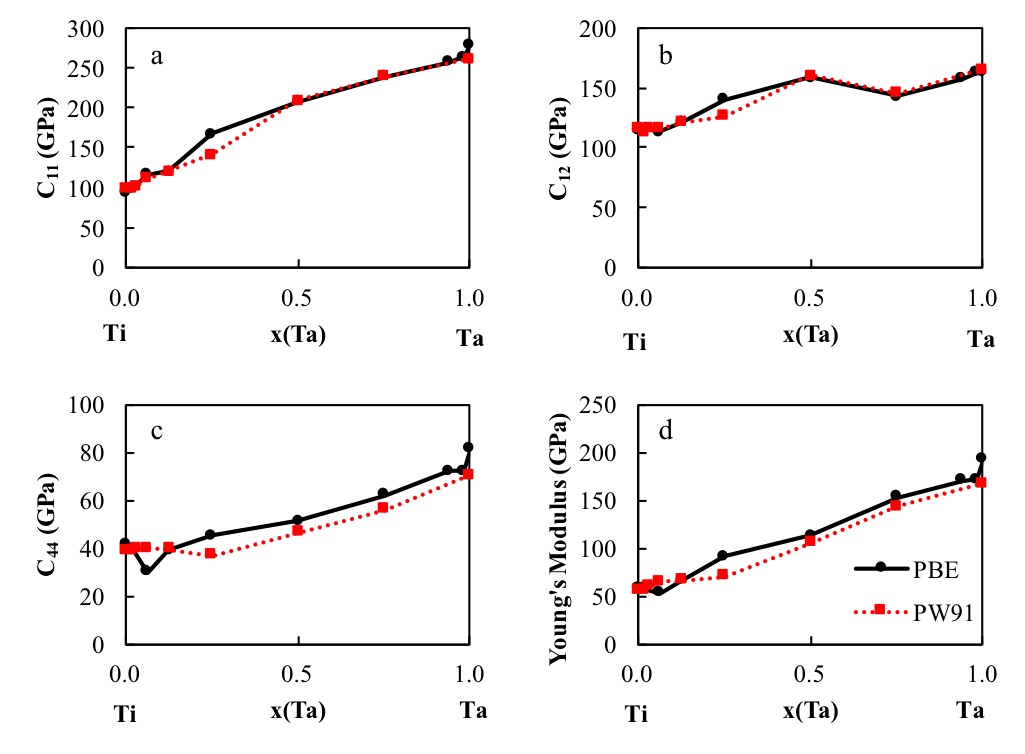
\includegraphics[width=\textwidth]{Chapter-2/Figures/PBEvsPW91.png}
	\caption{Elastic stiffness constants of the bcc Ti-Ta binary system calculated with the GGA and PBE exchange correction functions, respectively.}
	\label{Ch2-figure:PBEvsPW91}
\end{figure}
